\chapter{Implementation \& Evaluation}
\label{ch:impl_eval}

\begin{comment}
\section{Baseline with MCTS}
In order to develop a non-trivial strategy for an enemy playing the game(s) developed in chapter \ref{ch:modelling}, we'll use  the MCTS algorithm described in section \ref{sec:intro_mcts}.
While we could use MCTS in stead of MARL algorithms, MCTS does have some properties that make it unsuitable for our purposes. Firstly, it uses the complete state information of the game. Secondly, while it generally outperforms simpler algorithms like minimax, it still doesn't scale to more realistic situations. Furthermore, since MCTS works on turn-based games, the game from chapter \ref{ch:modelling} is adapted to accommodate executing actions in sequence for the two players.\\

However, it does allow us to develop strategies for two opposing players form the ground up. Thus using MCTS at this phase has two purposes:
\begin{enumerate}
    \item Analyzing the performance of the algorithm
    \item Obtaining a baseline opponent policy against which the MARL algorithms can be evaluated.
\end{enumerate}

\end{comment}
% ----------------------------------------------------------------------------------------

%\section{Innateness vs. Learned}
%\textbf{Discuss advantages / disadvantages of innate knowledge (e.g. no aim/fire when not in range $\rightarrow$ might be valid initial knowledge, while simple strategies might not)} 

\section{Notes on implementation}
This section describes a couple of technical points about the implementation of the algorithms.
\begin{itemize}
    \item Because of the structure of the observation that the environment provides to an agent (see \ref{sec:first_model}), all (learning) agents can use the same network. This is known as \emph{weight sharing} and improves the sample efficiency since only one common network must be trained instead of a network per agent.
    \item This network takes as input a tensor constructed from the observation and puts it through a fully-connected layer. The output for this layer is than fed to a GRU. At every time step, the hidden state of the GRU is transformed via another fully-connected layer in to the policy and/or the estimated $V$ or $Q$-values, depending on the type of algorithm. The entire network for an actor-critic agent, which does both value estimation as policy prediction, is schematically represented in figure \ref{fig:agent_net}. 
    \begin{figure}[htp]
        \centering
        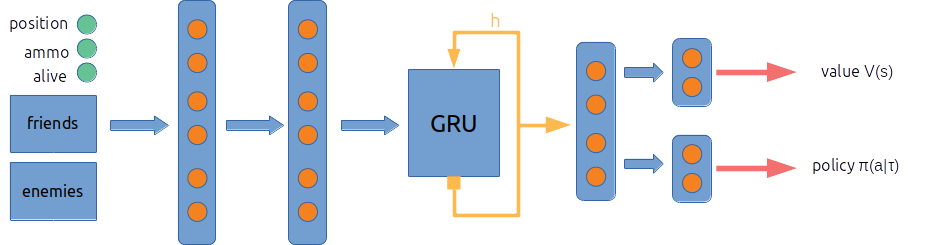
\includegraphics[width=14cm]{images/agent_net2.png}
        \caption{Actor-critic agent with a recurrent net}
        \label{fig:agent_net}
    \end{figure}
    \\A REINFORCE network only has the policy output. A Q-learning network outputs the Q-values for all potential actions.
    \item
        The output of a policy network is an array of numbers, one per possible action, computed by the final linear policy layer. These so-called \emph{logits} $l_i$ are transformed into probabilities $p(a_i | s)$ via a softmax function:
        \begin{equation}
            p(a_i | s) = \frac{e^{l_i}}{\sum_j e^{l_j}}
        \end{equation}
    \item In multi-agent settings, agents that have died no longer contribute to the game and the only action at their disposal is the {\tt do\_nothing} action. Care has been taken that for observations and actions that correspond to situations where the agent is dead are not used for the update process. Experiments have shown that neglecting to do this leads to inferior results.
    \item In Q-learning based algorithms like IQL and QMIX, the policy is created with the $\epsilon$-greedy action selection mechanism as described in section \ref{sec:deep_qn}. The $\epsilon$-term is responsible for the trade-off between exploration and exploitation. To assure enough exploration in the beginning, $\epsilon$ is typically reduced during training from its initial value of $1$ to a low final value like $0.05$. How this decrease of $\epsilon$ is done is determined by a scheduler which computes for each step in the learning process the corresponding value of $\epsilon$. In this project, an linear scheduler has been used.
    \item Algorithms of the Q-learning family, like IQL and QMIX, have more hyperparameters than algorithms from the policy gradient family due to the presence of a replay buffer and a target network. These hyperparameters includes the buffer and batch size, as well as the target synchronisation rate and the $\epsilon$ decay rate. This implies that searching an optimal combination of parameters becomes exponentially more difficult.
    \item In order to account for random effects, the average of the different measurements should be computed over multiple runs. However, this would mean that runs have to be repeated several times and development would slow down significantly. For this reason, averages were computed by letting a window slide over a single run and averaging the measurements in this window. This can be justified by the fact that the learning rate is chosen small enough so that the weights of the network don't change significantly in this window\footnote{Technically, we assume that the signal is weakly stationary and the ergodic hypothesis thus holds}.
    \item In all experiments, we used the ADAM variant of stochastic gradient descent. While the learning rate $\alpha$ is adapted during training by the algorithm as explained in section \ref{sec:deep_learning}, the initial value that we have to set can have a big impact on the convergence of the overall algorithm.
\end{itemize}

\section{Initial Model}
\subsection{Independent RL} % TODO bring IAC in line with definition of chapter 1
\label{sec:iql_applied}
This section discusses the application of IQL and IAC (section \ref{sec:intro_deep_indep_rl}) to the simple battlefield model described in section \ref{sec:first_model}. Two agents were trained with IQL and IAC (in casu the simple REINFORCE algorithm) on a 7-by-7 board against two opposing players who made random moves. The maximum range for all players was $5$ steps, so agents have to learn to approach other agents before firing. All training episodes were limited to maximum 100 steps.\\

A comment on random opponents: agents that make random moves are indeed simple to beat; the final goal however is to work in an iterative fashion: 
\begin{enumerate}
    \item Train two agents against two random agents.
    \item Train two new agents against these two already trained agents until they can consistently beat them.
    \item Continue in this way until no more progress is made.
\end{enumerate}
Some results of this procedure will be discussed in section \ref{sec:model_transfer}.
% Nov13_10-05-55_ideapad-pg smoothing 0.95
% Add (insert): run 171
% [21Jan20] -> experiment 3 - run 187

This paragraph describes the results for independent REINFORCE. The training of both agents was run for 50000 episodes, generated by sampling actions from the policy $\pi_i(a_t|s_t)$ and interacting with the environment.\\
First, lets compare the gradients of the loss function. As explained in section \ref{sec:intro_policy_grads}, these gradients will drive the weights of the network to their optimal values. Figures \ref{fig:exp1_grad0} and \ref{fig:exp1_grad1} show how the $L2$-norm\footnote{The $L2$-norm is the square-root of the sum-of-squares of the gradients $\sqrt{\sum_i \nabla_{\bm{\theta}} J_{i}(\bm{\theta})^2}$}  of each policy gradient $G_t \, \nabla_{\bm{\theta}} \ln \pi(A_t|S_t,\bm{\theta})$ evolves during training for both agents. This norm gives an indication how the gradient ascent algorithm changes the network parameters. Notice that while initially the gradient increases, it finally tops off and starts to decrease. Running the experiment longer will show both graphs converging to zero, meaning that the agents have reached their goal and are no longer learning.\\
As explained previously, these curves are computed by taking the average over a moving window. The shaded area represents the confidence interval around the average value.
\begin{figure}
\centering
\begin{minipage}{.5\textwidth}
  \centering
  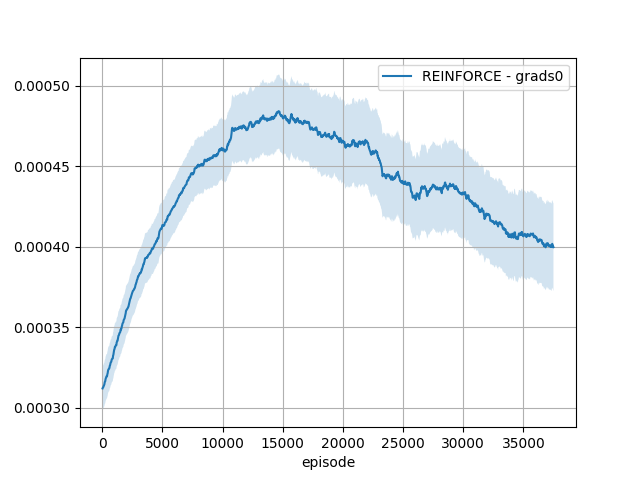
\includegraphics[width=8cm]{images/experiment4/grad0.png}
  \captionof{figure}{Gradient estimate for agent $0$}
  \label{fig:exp1_grad0}
\end{minipage}%
\begin{minipage}{.5\textwidth}
  \centering
  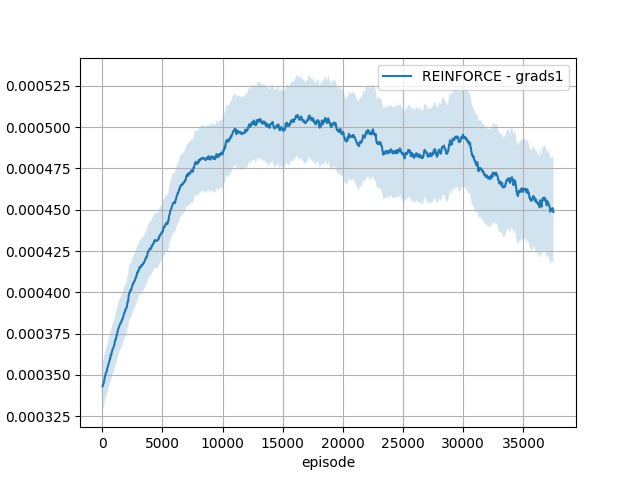
\includegraphics[width=8cm]{images/experiment4/grad1.png}
  \captionof{figure}{Gradient estimate for agent $1$}
  \label{fig:exp1_grad1}
\end{minipage}
\end{figure}

Figure \ref{fig:exp1_length} shows the average duration of an episode. Notice that initially, when the agent's policy network has random weights and the agent effectively behaves as a random agent, the episodes take a long time because nobody is taking any directed actions. Once the agent's learns from experience, his behavior becomes more directive and the episode duration decreases rapidly. This behavior is encouraged by the fact that the agent receives a small negative reward for every step, incentivizing the agents to reduce the episode length. Figure \ref{fig:exp1_reward} shows the average final reward per episode for the agents\footnote{This is not the cumulative reward, and thus doesn't take into account any negative step rewards}. Initially, the agents lose as often as they win; the reward is negative, partially because agents are penalized for draws (e.g. because they run out of ammo). However, the win rate increases rapidly and finally the agents will win always all the time. This curve is called the \emph{learning curve} and will be the standard way to evaluate the performance of a MARL algorithm.\\

\begin{figure}
\centering
\begin{minipage}{.5\textwidth}
  \centering
  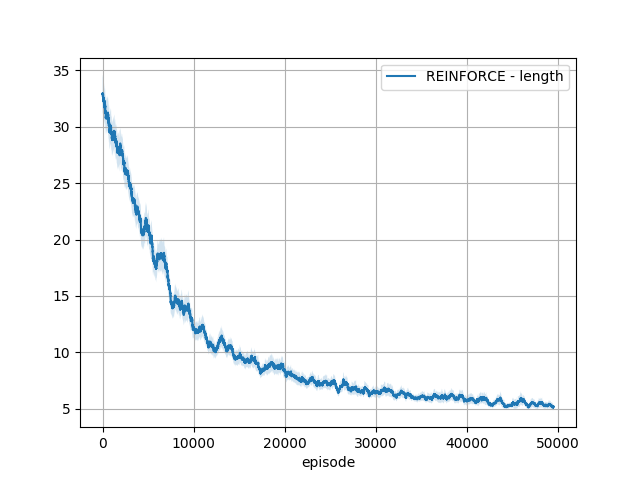
\includegraphics[width=8cm]{images/experiment4/mean_length.png}
  \captionof{figure}{Mean episode length}
  \label{fig:exp1_length}
\end{minipage}%
\begin{minipage}{.5\textwidth}
  \centering
  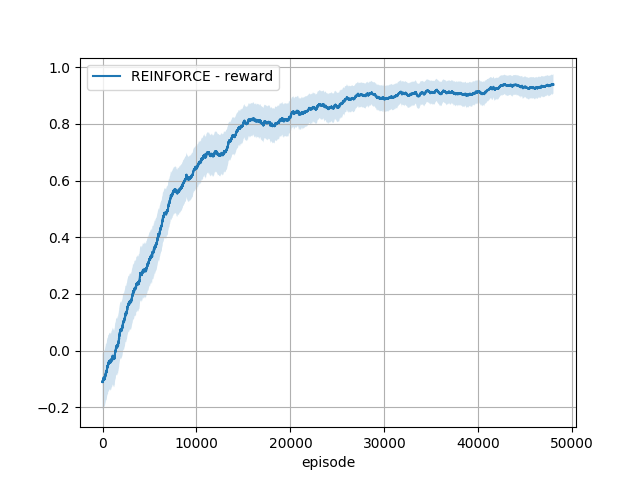
\includegraphics[width=8cm]{images/experiment4/mean_reward.png}
  \captionof{figure}{Mean reward for agents of team 1}
  \label{fig:exp1_reward}
\end{minipage}
\end{figure}

In this simple scenario, the agents have learned to (in this order):
\begin{enumerate}
    \item Aim at the opposing agents (resp. $0 \rightarrow 2$ and $1 \rightarrow 3$).
    \item Come closer until the opposing agent is in range.
    \item Fire once the opposing agent is in range.
\end{enumerate}
Figure \ref{fig:simple_tactic01} shows how this is done. A white line between agents means one agent is aiming at the other. The actions undertaken by the four agents is shown in the top left corners.

%\includemovie{8cm}{8cm}{images/tactic01.gif}
% \begin{frame}{}
%   \animategraphics[loop,controls,width=10cm]{10}{images/animation01/screenshot0-}{0}{4}
% \end{frame}

% \begin{frame}
%     \transduration<0-4>{0}
%     \multiinclude[<+->][format=png, graphics={width=10cm}]{images/animation01/screenshot0}
% \end{frame}

\begin{figure}
\centering
\begin{minipage}{.5\textwidth}
  \centering
  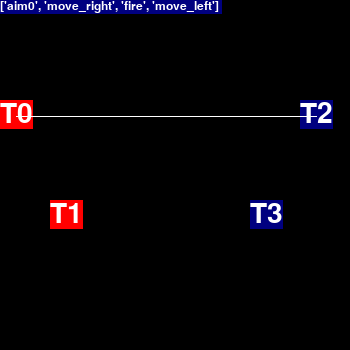
\includegraphics[width=7cm]{images/animation01/screenshot0-1.png}
\end{minipage}%
\begin{minipage}{.5\textwidth}
  \centering
  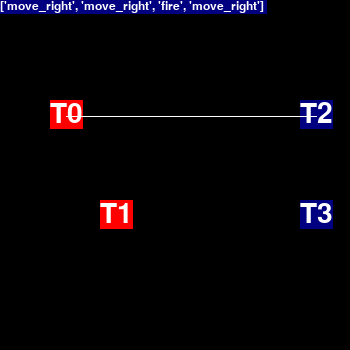
\includegraphics[width=7cm]{images/animation01/screenshot0-2.png}
\end{minipage}
%\end{figure}
%\begin{figure}
\centering
\begin{minipage}{.5\textwidth}
  \centering
  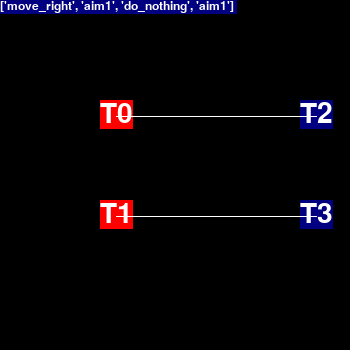
\includegraphics[width=7cm]{images/animation01/screenshot0-3.png}
\end{minipage}%
\begin{minipage}{.5\textwidth}
  \centering
  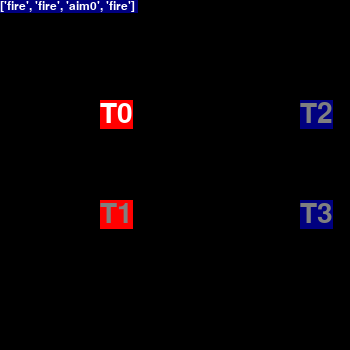
\includegraphics[width=7cm]{images/animation01/screenshot0-4.png}
\end{minipage}
\caption{A simple learned tactic}
\label{fig:simple_tactic01}
\end{figure}

Next, we compare the learning curves of the three types of independent learning algorithms: (i) REINFORCE, (ii) Independent Actor-Critic (IAC) and (3) Independent Q-Learning (IQL). The resulting learning curves are represented in figure \ref{fig:compare_reward} for games where 2 learning agents play against 2 random agents.

\begin{figure}[htp]
    \centering
    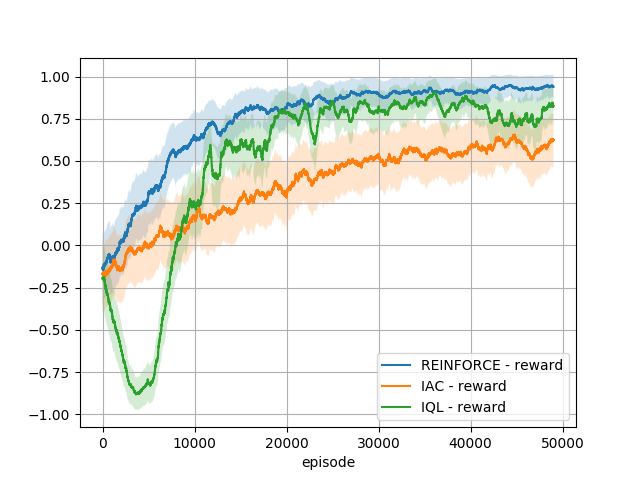
\includegraphics[width=14cm]{images/experiment4/compare_reward.png}
    \caption{Learning rate for REINFORCE, IAC and IQL for 2v2 games}
    \label{fig:compare_reward}
\end{figure}

The following points are significant:
\begin{itemize}
    \item Out of the 3 algorithms, REINFORCE works best.
    \item IQL initially goes in the wrong direction (i.e. makes wrong moves) before starting to improve the reward. This is caused by the high initial $\epsilon$ in the $\epsilon$-greedy action selection process which causes the behavior to be random instead of guided by the learned $Q$-values.
    \item Since IQL derives the policy from the learned $Q$-values, its behavior during learning undergoes significantly higher variation than REINFORCE. This is because gradual changes in $\hat Q$ can lead to suddenly preferring one action over another.
    \item The learning curve of IAC is slower than those for REINFORCE and IQL. This is probably because IAC has to learn both a policy and value-estimation function at the same time.
    \item IAC is highly dependent on the inclusion of an entropy-term to avoid the policy distribution from collapsing to a distribution that puts all probability mass on a single action.
\end{itemize}

Independent REINFORCE definitely works best, and this has been confirmed by numerous experiments. IQL can be an alternative, but as mentioned above, many hyperparameters have to be tuned to achieve good performance. This point will also be addressed when discussing QMIX. IAC performs significantly worse than independent REINFORCE. Why this is the case shall be part of further investigations.\\
In the next section the performance of QMIX will be compared against REINFORCE.

\begin{comment}
\textbf{TODO:} Rephrase the paragraph below.\\
The next evolution is to represent the agent as a recurrent neural network as explained in section \ref{sec:deep_pg}. The input of the network are the two major components of the state vector $\bm{s_t}$:
\begin{enumerate}
    \item The game board, namely the actual position of the agent relative to the board and each other, and
    \item Additional information about the agents (are they alive? What is the ammo level?)
\end{enumerate}
The board information is well suited to serve as input of a convolutional layer, since it contains spatial information. The additional information on the other hand will be fed to a fully-connected neural network layer. The result of both these layers is then combined and serves as the input for the a fully-connected layer. The output of this layer is then fed to a GRU. The neural net will have two heads, as explained in section \ref{sec:deep_pg}, and can thus be used in an actor-critic algorithm. An overview of the agent's neural network is shown in figure \ref{fig:agent_net}.
\begin{figure}[htp]
    \centering
    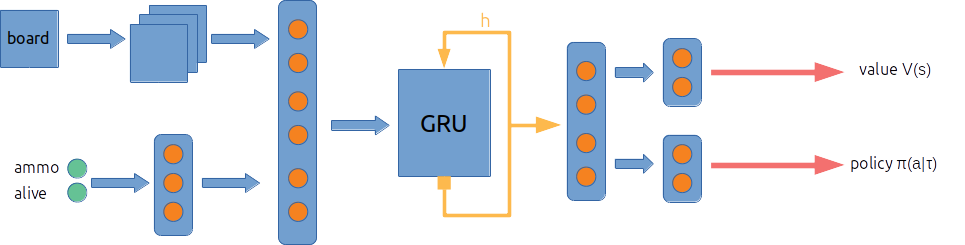
\includegraphics[width=16cm]{images/agent_net.png}
    \caption{Actor-critic agent with recurrent net}
    \label{fig:agent_net}
\end{figure}

While this modification might result in a theoretical improvement, this is not the case in practice. Figure \ref{fig:newplot194_195} shows the learning curve for agents with non-recurrent (blue) and recurrent neural nets (green). While both learn a winning strategy, it is not feasible to say one approach is better than the other. \textbf{TODO}: improve this (correct or explain).

% comparison 194-195
\begin{figure}[htp]
    \centering
    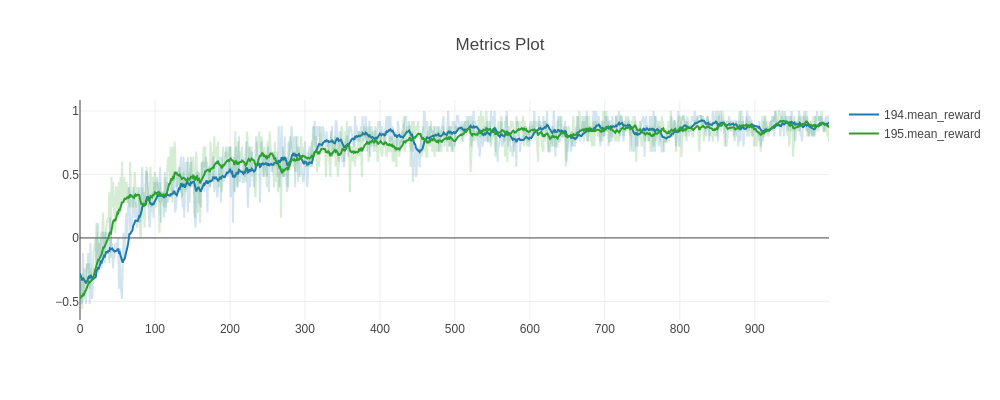
\includegraphics[width=14cm]{images/experiment2/newplot194_195.png}
    \caption{Forward vs. GRU Network}
    \label{fig:newplot194_195}
\end{figure}

%insert comparison PG (run ideapad 582) and IQL (run ideapad 590)
\end{comment}

\subsection{QMIX}
As explained in section \ref{sec:intro_qmix}, QMIX is an algorithm of the Q-learning family that combines the Q-value estimate of the different agents into a $Q_{tot}$ such that $\frac{\partial Q_{tot}}{\partial Q_i} \geq 0$ for all agents $i$. This guarantees that when each agent chooses his best action $a_i$, the combined action set $[a_1 \ldots a_N]$ will also be the best possible joint action for the team.\\
QMIX uses during training the state information $s_t$ to set the weights of the mixing network in figure \ref{fig:qmix_structure}. To do this, the state information was transformed in a tensor of size {\tt n\_agents x 5}, where each agent is represented by 5 items: his position $(x, y)$, whether he is still alive, his ammo level and at whom he is aiming at (if that is the case).\\
Figure \ref{fig:comp_qmix_pg} compares the learning curve of REINFORCE with the one for QMIX.
% comparison 396-419
\begin{figure}[htp]
    \centering
    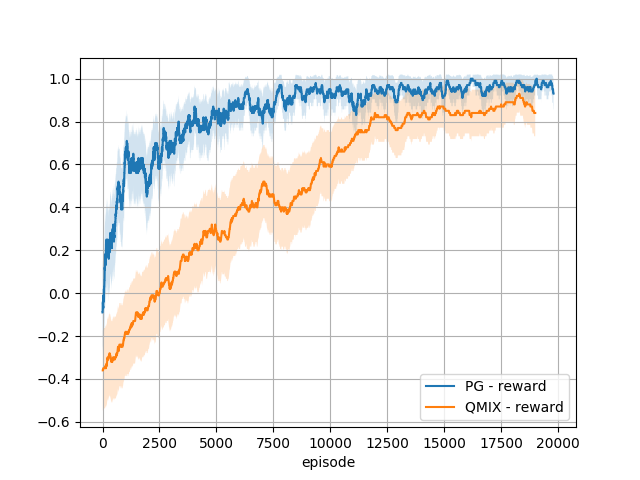
\includegraphics[width=14cm]{images/experiment5/pg_v_qmix_simple.png}
    \caption{QMIX vs independent REINFORCE in a simple environment}
    \label{fig:comp_qmix_pg}
\end{figure}
Both algorithms convergence to a situation where the blue teams wins the large majority of its games. However, independent REINFORCE clearly works better, both in sample efficiency (since its curve is steeper) and in final result. Indeed, investigation of the resulting strategies didn't show anything better than REINFORCE produced. However, QMIX is an algorithm that encourages cooperation between agents and its advantages should become clearer when we look at the extended environment.\\
Experimentation has shown a few remarkable facts:
\begin{enumerate}
    \item The discount factor $\gamma$ is a critical parameter: policy gradient algorithms like REINFORCE and IAC require a high $\gamma$ (around $0.99$), while Q-learning based algorithms like IQL and QMIX only converge when $\gamma$ is lower ($0.8$ and below). A possible reason might be that PG algorithms base their update on a sequence of steps of a single episode, while Q-learning algorithms take random samples out a buffer of steps coming from multiple episodes. This means that the temporal effect of actions is more pronounced for PG and this can have an impact on the sensitivity on $\gamma$. However, this explanation has not been confirmed.
    \item Convergence of QMIX is much better when the step penalty is increased and the maximum episode length is kept low. REINFORCE in turn has no problem to converge with a lower (or even zero) step penalty.
\end{enumerate}

\section{Extended Model}
This section describes the obtained results when the different algorithms are applied to the second model of which the characteristics were sketched in section \ref{sec:extended_model}.
\subsection{Independent RL}
\subsection{QMIX}

\section{Model Transfer}
\label{sec:model_transfer}
Obtaining a model that performs well against an opponent that deploys a random strategy is one thing. More interesting thing can happen when we train against a more advanced agents. To do so, the neural network and its inputs on which an agent relies to chose his action has been constructed in such a way that:
\begin{itemize}
    \item agents of the same team share the same network (weight sharing), and
    \item agents of the opposing team can reuse that trained network to obtain the same performance 
\end{itemize}
In this way, we can swap the trained network from the blue team to the red one to get an opponent that doesn't behave randomly but uses a slightly smarter strategy. By doing this in an iterative fashion we make continuously improve our strategy. More concretely:
\begin{enumerate}
    \item Start training the blue team against a random opponent;
    \item After a certain number of steps or once the blue team consistently beats the red one, transfer the network from the blue team to the red one;
    \item Continue improving the blue team against the better opponent. Either start from a clean network or keep the already trained network. The former option might be useful to avoid getting stuck in a local minimum where the learned strategy is too brittle and only works in a limited number of cases. The latter option is obviously more sample efficient.
    \item Go back to step 2.
\end{enumerate}

\begin{figure}[htp]
    \centering
    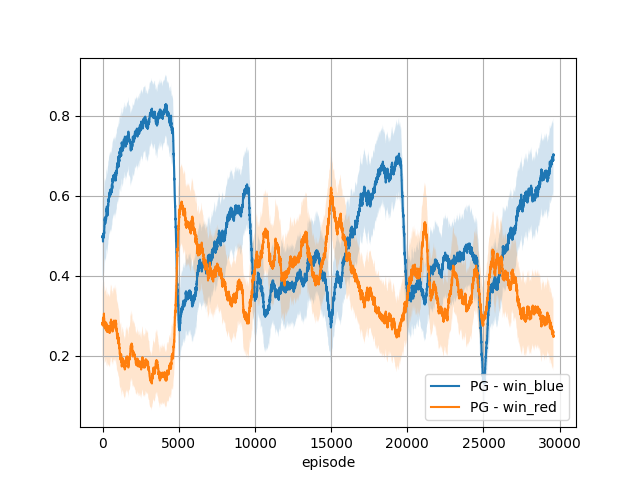
\includegraphics[width=14cm]{images/iteration/iterative.png}
    \caption{Sequence of model transfers from team blue to team red}
    \label{fig:iteration}
\end{figure}
Figure \ref{fig:iteration} shows the win rate for both blue and red teams where after each 5000 episodes the network was transferred to the red team and the agents from the blue team restart training as random agents. During some cycles (e.g. from episode 10000 to 15000) it is hard to overcome the opponent while during other cycles the blue team easily overcomes the red one (e.g. from episode 15000 to 20000).



% TODO: explain model transfering from friend to foe
% TODO (maybe) discuss transferability over different terrains
% python3 qmix.py with gamma=0.9 qmix_ns=True max_episode_length=20 step_penalty=0.1 lr=0.001 % n_steps=50000 > /dev/null &
